%Dokumentenklasse "scrbook" - Erweitert um den Verweis auf die Verzeichnisse und Texteigenschaften
\documentclass[chapterprefix=true, 12pt, a4paper, oneside, parskip=half, listof=totoc, bibliography=totoc, numbers=noendperiod]{scrbook}

% Ränder (Standard bottom ca. 52mm anbzüglich von ca. 4mm für die nach oben rechts gewanderte Seitenzahl)
%Anpassung der Seitenränder
\usepackage[bottom=32mm,left=25mm,right=25mm]{geometry}

% Ränder bei Bedarf zeigen
%\usepackage{showframe}

%Tweaks für scrbook
\usepackage{scrhack}

%Blindtext
\usepackage{blindtext}

%Erlaubt unteranderem Umbrücke captions
\usepackage{caption}

%Stichwortverzeichnis
\usepackage{imakeidx}

%Kompakte Listen
\usepackage{paralist}

%Zitate besser formatieren und darstellen
\usepackage{epigraph}

%Glossar + Stichworverzeichnis
\usepackage[toc, acronym]{glossaries} % Akronyme werden als eigene Liste aufgeführt
\glsenablehyper

%Anpassung von Kopf- und Fußzeile
%beinflusst die erste Seite des Kapitels
\usepackage[automark,headsepline]{scrlayer-scrpage}
\automark{chapter}
\ihead{\leftmark}
\chead{}
\ohead{\thepage}
\ifoot*{}
\cfoot[\thepage]{}
\cfoot*{}
\ofoot*{}
\pagestyle{scrheadings}

%Auskommentieren für die Verkleinerung des vertikalen Abstandes eines neuen Kapitels
%\renewcommand*{\chapterheadstartvskip}{\vspace*{.25\baselineskip}}

%Zeilenabstand 1,5
\usepackage[onehalfspacing]{setspace}

%Verbesserte Darstellung der Buchstaben zueinander
\usepackage[stretch=10]{microtype}

%Deutsche Bezeichnungen für angezeigte Namen (z.B. Innhaltsverzeichnis etc.)
\usepackage[ngerman]{babel}

%Unterstützung von Umlauten und anderen Sonderzeichen (UTF-8)
\usepackage{lmodern}
\usepackage[utf8]{luainputenc}
\usepackage[T1]{fontenc}

%Einfachere Zitate
\usepackage{epigraph}

%Verwendung von Akronymen
\usepackage[printonlyused]{acronym}

%Unterstützung der H positionierung (keine automatische Verschiebung eingefügter Elemente)
\usepackage{float} 

%Erlaubt Umbrüche innerhalb von Tabellen
\usepackage{tabularx}

%Erlaubt Seitenumbrüche mit Tabellen
\usepackage{longtable}

%Erlaubt die Darstellung von Sourcecode mit Highlighting
\usepackage{listings}

%Definierung eigener Farben bei nutzung eines selbst vergebene Namens
\usepackage[table,xcdraw]{xcolor}

%Vektorgrafiken tikz
\usepackage{tikz}

%Grafiken (wie jpg, png, etc.)
\usepackage{graphicx}

%Grafiken von Text umlaufen lassen
\usepackage{wrapfig}

%Grafik bestehend aus mehreren Grafiken
\usepackage{subfigure}

%Ermöglicht Verknüpfungen innerhalb des Dokumentes (e.g. for PDF), Links werden durch "hidelink" nicht explizit hervorgehoben
\usepackage[hidelinks,ngerman]{hyperref}

%Einbindung und Verwaltung von Literaturverzeichnissen
\usepackage{csquotes} %wird von biber benötigt
\usepackage[style=alphabetic, backend=biber, bibencoding=utf8]{biblatex}
\addbibresource{references/references.bib}

%enable the macro \mathbb
\usepackage{amssymb}
\usepackage{amsmath}

%-------------------------------Zusätzliche Anpassungen und Modifikationen--------------------------------------------%

%Anpassung der Überschriften
\addtokomafont{disposition}{\rmfamily}

%Zusätzliche Farben
\definecolor{Ao}{rgb}{0.0, 0.39, 0.0}
\definecolor{antiquefuchsia}{rgb}{0.57, 0.36, 0.51}
\definecolor{bostonuniversityred}{rgb}{0.8, 0.0, 0.0}

% Padding für images innerhalb von longtables
\usepackage{verbatimbox}
\newcommand\Includegraphics[2][]{\addvbuffer[5pt 0pt]{\includegraphics[#1]{#2}}}

%Umbenennungen
\renewcommand{\lstlistlistingname}{Source Code Content}

%Pluszeichen in der Reference beim zitieren ausblenden
\renewcommand*{\labelalphaothers}{}

%Anpassugen zur Quelltextdarstellung, kann bei Bedarf überschrieben werden (z.B. wenn unterschiedliche Sprachen zum Einsatz kommen)
\renewcommand{\lstlistingname}{Code snippet}
\lstset{
	language=python,
	numbers=left,
	columns=fullflexible,
	aboveskip=5pt,
	belowskip=10pt,
	basicstyle=\small\ttfamily,
	backgroundcolor=\color{black!5},
	commentstyle=\color{black},
	morecomment=[s]{.s}{hape}, % workaround to exclude ".shape"
	keywordstyle=\color{antiquefuchsia},
	otherkeywords={self, else},
	emphstyle=\color{bostonuniversityred},
	emph={shape,units,name,filters,kernel_size,activation,padding,kernel_initializer,kernel_regularizer,bias_initializer,inputs,outputs,mode,distribution,minval,maxval, callback_args, low, high, limit, window_length, size, mu, theta, sigma},
	stringstyle=\color{Ao},
	showspaces=false,
	showstringspaces=false,
	showtabs=false,
	xleftmargin=16pt,
	xrightmargin=0pt,
	framesep=5pt,
	framerule=1pt,
	frame=leftline,
	rulecolor=\color{black},
	tabsize=2,
	breaklines=true,
	breakatwhitespace=true
}

%Anpassungen für das Abkürzungsverzeichnis
\newglossarystyle{dottedlocations}{%
	\glossarystyle{list}%
	\renewcommand*{\glossaryentryfield}[5]{%
		\item[\glsentryitem{##1}\glstarget{##1}{##2}] \emph{##3}%
		\unskip\leaders\hbox to 2.9mm{\hss.}\hfill##5}%
	\renewcommand*{\glsgroupskip}{}%
}

% Titles Config - CHOOSE ONE section for title format

%% Used for titleGraduation Bachelor
%% Based on https://ai-bachelor.htw-berlin.de/files/Stg/AI/richtlinie_ba-arbeit_ai_06_02_13.pdf
\makeatletter

\newcommand*{\gradeType}[1]{\gdef\@gradeType{#1}}
\newcommand*{\firstExaminer}[1]{\gdef\@firstExaminer{#1}}
\newcommand*{\secondExaminer}[1]{\gdef\@secondExaminer{#1}}
\newcommand*{\matrikelnr}[1]{\gdef\@matrikelnr{#1}}
\newcommand*{\submitDate}[1]{\gdef\@submitDate{#1}}

\renewcommand*{\maketitle}{
	\begin{titlepage}
		\newgeometry{left=2.5cm,right=2.5cm,top=2.5cm,bottom=2.5cm}
		\begin{figure}[H]
			\centering
			
\includegraphics[width=0.5\textwidth]{resources/htw/logo}
		\end{figure}
		\begin{center}
			\vfill
			{\Large \@title\par}
			\vskip 0.5cm
			{\large \bfseries Abschlussarbeit\par}
			\vskip 0.5cm
			{\large zur Erlangung des akademischen Grades\vskip 0.5cm \bfseries \@gradeType}
			\vskip 0.5cm
			{\large an der}
			\vskip 0.5cm
			{\large Hochschule für Technik und Wirtschaft Berlin}
			\vskip 0.0cm
			{\large Fachbereich Wirtschaftswissenschaften II}
			\vskip 0.0cm
			{\large Studiengang Angewandte Informatik}
			\vfill
			\begin{flushleft}
				\begin{tabular}[t]{rl}
					1. Prüfer: &\@firstExaminer\\
					2. Prüfer: & \@secondExaminer\\
					\\
					Eingereicht von: &\@author\\
					Immatrikulationsnummer: & \@matrikelnr\\
					Eingereicht am: & \@submitDate
				\end{tabular}
			\end{flushleft}
		\end{center}
		\restoregeometry
	\end{titlepage}
}
\makeatother
\gradeType{Bachelor of Science (B.Sc.)}
\secondExaminer{TODO}

%% Used for titleGraduation Master
%% Based on https://ai-master.htw-berlin.de/files/Stg/AI/richtlinie_ma-arbeit_ai_25_01_13.pdf
%\makeatletter

\newcommand*{\gradeType}[1]{\gdef\@gradeType{#1}}
\newcommand*{\firstExaminer}[1]{\gdef\@firstExaminer{#1}}
\newcommand*{\secondExaminer}[1]{\gdef\@secondExaminer{#1}}
\newcommand*{\matrikelnr}[1]{\gdef\@matrikelnr{#1}}
\newcommand*{\submitDate}[1]{\gdef\@submitDate{#1}}

\renewcommand*{\maketitle}{
	\begin{titlepage}
		\newgeometry{left=2.5cm,right=2.5cm,top=2.5cm,bottom=2.5cm}
		\begin{figure}[H]
			\centering
			
\includegraphics[width=0.5\textwidth]{resources/htw/logo}
		\end{figure}
		\begin{center}
			\vfill
			{\Large \@title\par}
			\vskip 0.5cm
			{\large \bfseries Abschlussarbeit\par}
			\vskip 0.5cm
			{\large zur Erlangung des akademischen Grades\vskip 0.5cm \bfseries \@gradeType}
			\vskip 0.5cm
			{\large an der}
			\vskip 0.5cm
			{\large Hochschule für Technik und Wirtschaft Berlin}
			\vskip 0.0cm
			{\large Fachbereich Wirtschaftswissenschaften II}
			\vskip 0.0cm
			{\large Studiengang Angewandte Informatik}
			\vfill
			\begin{flushleft}
				\begin{tabular}[t]{rl}
					1. Prüfer: &\@firstExaminer\\
					2. Prüfer: & \@secondExaminer\\
					\\
					Eingereicht von: &\@author\\
					Immatrikulationsnummer: & \@matrikelnr\\
					Eingereicht am: & \@submitDate
				\end{tabular}
			\end{flushleft}
		\end{center}
		\restoregeometry
	\end{titlepage}
}
\makeatother
%\gradeType{Master of Science (M.Sc.)}
%\secondExaminer{TODO}

%% Used for titleResearchProject
%% Based on http://christianherta.de/lehre/HTW/richtlinie-wissenschaftliche-Arbeiten.pdf
%\makeatletter

\newcommand*{\firstExaminer}[1]{\gdef\@firstExaminer{#1}}
\newcommand*{\subTitle}[1]{\gdef\@subTitle{#1}}
\newcommand*{\researchPart}[1]{\gdef\@researchPart{#1}}
\newcommand*{\matrikelnr}[1]{\gdef\@matrikelnr{#1}}
\newcommand*{\submitDate}[1]{\gdef\@submitDate{#1}}


\renewcommand*{\maketitle}{
	\begin{titlepage}
		\newgeometry{left=2.5cm,right=2.5cm,top=2.5cm,bottom=2.5cm}
		\begin{figure}[H]
			\centering
			
\includegraphics[width=0.5\textwidth]{resources/htw/logo}
		\end{figure}
		\begin{center}
			\vfill
			{\Large \@title\par}
			\vskip 0.5cm
			{\large \bfseries Forschungsprojekt \@researchPart\par}
			\vskip 0.5cm
			{\large an der}
			\vskip 0.5cm
			{\large Hochschule für Technik und Wirtschaft Berlin}
			\vskip 0.0cm
			{\large Fachbereich Wirtschaftswissenschaften II}
			\vskip 0.0cm
			{\large Studiengang Angewandte Informatik}
			\vfill
			\begin{flushleft}
				\begin{tabular}[t]{rl}
					Supervisor: &\@firstExaminer\\
					\\
					Submitted by: &\@author\\
					Matriculation Number: & \@matrikelnr\\
					Submission Date: & \@submitDate
				\end{tabular}
			\end{flushleft}
		\end{center}
		\restoregeometry
	\end{titlepage}
}
\makeatother
%\researchPart{A/B} % choose A or B

% Titles Config End

% Used by all titles
\title{Titel der Arbeit}
\author{Konstantin Bruckert}
\matrikelnr{s0XXXXXX}
\submitDate{XX.XX.2018}
\firstExaminer{Prof. Dr. V. Nachname}
% End Titles

\makeindex[title=Index, options=-s indexstyle.ist, intoc]
\indexsetup{level=\chapter*,toclevel=chapter}

\makenoidxglossaries
\loadglsentries{glossary_and_acronyms.tex}
\setacronymstyle{long-short}
\begin{document}

\pagenumbering{alph} % fix for same identifier warning, character is not show in title
\maketitle

\pagenumbering{roman}
\chapter*{Vorwort}
TODO
Testen des Vorwortes \clearpage  % FOR BA/MA-THESIS, NOT REQUIRED FOR RESEARCHPROJECT
\chapter*{Kurzbeschreibung}
TODO
\\
\\
\textbf{Schlagworte:} TODO \clearpage

\tableofcontents \newpage

\pagenumbering{arabic}
\chapter{Einleitung}
Beispiel Quellen:
\\
wissenschaftlich \cite{doi:10.1162/neco.1989.1.4.541}
\\
Onlinequelle \cite{LSVRC}
\\
git \cite{chollet2015}
\\
Beispiel für Glossar \gls{api}

\section{Motivation}
TODO

\section{Zielsetzung}
TODO

\section{Vorgehensweise und Aufbau der Arbeit}
TODO \clearpage
\chapter{Grundlagen}
TODO

\section{Beispiel Unterkapitel} 
Beispiel Abbildung \ref{img:cnn_example_network} mit Zitat.
\begin{figure}[H]
	\centering
	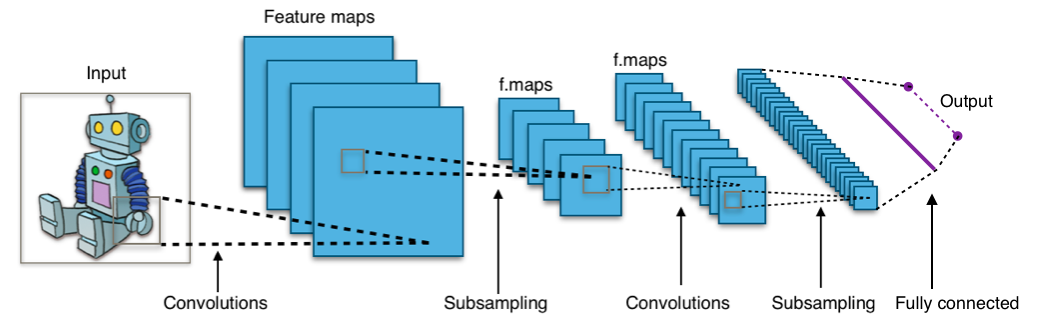
\includegraphics[width=0.95\textwidth]{resources/cnn/typical_cnn}
	\caption{Beispiel CNN Arhcitektur \cite{typical_cnn_img}}
	\label{img:cnn_example_network}
\end{figure}

\section{Verwandte Arbeiten}
TODO \clearpage
\chapter{Analyse}
Robot Operating System \cite{288}
\newline
Tensorflow \cite{Abadi:2016:TSL:3026877.3026899}

\section{Beispiel Unterkapitel}
TODO

\section{Beispiel Unterkapitel}
TODO \clearpage
\chapter{Konzeption}
TODO

\section{Prior Work TODO}
nur benötigt, wenn die Arbeit auf einer vorherigen aufbaut.

\section{Beispiel Unterkapitel}
TODO

\subsection{Beispiel Unterkapitel zweiter Ebene}
Formelbeispiel
\begin{equation}
	\pi_\theta(s, a) = P [a | s, \theta]
\end{equation}
wobei, $s$ den Zustand repräsentiert, $a$ die Aktion und $\theta$ ... \clearpage
\chapter{Implementierung}
\label{cha:implmentation}
Code Biespiel and Referenze: Code \ref{lst:tf_graph_save}. Nicht geeignet für große Code Biespiele. Verwenden Sie hierfür dne Anhang. Lediglich sehr relevante Kurzzeiler können auf diese Weise dargestellt werden. 
\begin{lstlisting}[caption={Klasse Agent - Tensorflow Graph}, captionpos=b, label={lst:tf_graph_save}]
from keras import backend as k
...
def __init__(...):
	...
	self.graph = k.get_session().graph
	...
\end{lstlisting}

\section{Beispiel Unterkapitel}
TODO

\section{Beispiel Unterkapitel}
TODO \clearpage
\chapter{Test}
TODO

\section{Beispiel Unterkapitel}
TODO

\section{Beispiel Unterkapitel}
TODO \clearpage
\chapter{Evaluation}
\label{sec:evaluation}
TODO

\section{Beispiel Unterkapitel}
Beispiel einer Tabelle:
\begin{longtable}{|c|c|c|c|}
	\hline
	\multicolumn{1}{|c}{\textbf{Spalte 1}} &
	\multicolumn{1}{|c}{\textbf{Spalte 2}} &
	\multicolumn{1}{|c|}{\textbf{Spalte 3}} \\
	\hline
	\endfirsthead
	
	\multicolumn{3}{c}{Beschreibung}\\ \hline
	\multicolumn{1}{|c}{\textbf{Spalte 1}} &
	\multicolumn{1}{|c}{\textbf{Spalte 2}} &
	\multicolumn{1}{|c|}{\textbf{Spalte 3}} \\
	\hline
	\endhead
	
	\multicolumn{2}{c}{Fortsetzugn auf der nächsten Seite}
	\endfoot
	
	\caption{Beschreibung}
	\label{tab:example}
	\endlastfoot
	
	TODO & TODO & TODO \\ \hline
	TODO & TODO & TODO  \\ \hline
\end{longtable}

\section{Beispiel Unterkapitel}
TODO \clearpage
\chapter{Fazit}
TODO

\section{Zusammenfassung}
TODO

\section{Kritischer Rückblick}
TODO (Reflexion und Bewertung der Zielsetzung gegenüber erreichtem Ergebnis)

\section{Ausblick}
TODO \clearpage

\pagenumbering{Roman}
% List of Figures
\listoffigures \clearpage
% List of Tables
\listoftables \clearpage
% Source Code Content
\lstlistoflistings \clearpage

\printindex \clearpage

\printnoidxglossary[title=Glossar] \clearpage

\defbibfilter{scientific}{
	type=article or
	type=inbook or
	type=book or
	type=unpublished or
	type=inproceedings or
	type=incollection or
	type=manual or
	type=phdthesis
}

\printbibliography[heading=bibintoc, filter=scientific, title={Literaturverzeichnis}]\clearpage
\printbibliography[heading=bibintoc, keyword={online}, title={Onlinereferenzen}]\clearpage
\printbibliography[heading=bibintoc, keyword={image}, title={Bildreferenzen}]\clearpage

% Appendix
\appendix
\chapter{}
\addcontentsline{toc}{chapter}{Anhang A}
\section{Beispiel}
\label{code:appendix_example}
TODO

% Eigenständigkeitserklärung (CHOOSE ONE)
\addchap{Eigenständigkeitserklärung}

Hiermit versichere ich, dass ich die vorliegende Bachelorarbeit selbstständig und nur unter Verwendung der angegebenen Quellen und Hilfsmittel verfasst habe. Die Arbeit wurde bisher in gleicher oder ähnlicher Form keiner anderen Prüfungsbehörde vorgelegt.

\vskip 1cm

Berlin, den XX.XX.2018

\vskip 1.5cm

Vorname Nachname
 % FOR BACHELORTHESIS
%\addchap{Eigenständigkeitserklärung}

Hiermit versichere ich, dass ich die vorliegende Masterarbeit selbstständig und nur unter Verwendung der angegebenen Quellen und Hilfsmittel verfasst habe. Die Arbeit wurde bisher in gleicher oder ähnlicher Form keiner anderen Prüfungsbehörde vorgelegt.

\vskip 1cm

Berlin, den XX.XX.2018

\vskip 1.5cm

Vorname Nachname
 % FOR MASTERTHESIS
%\addchap{Eigenständigkeitserklärung}

Hiermit versichere ich, dass ich die vorliegende Arbeit selbstständig und nur unter Verwendung der angegebenen Quellen und Hilfsmittel verfasst habe. Die Arbeit wurde bisher in gleicher oder ähnlicher Form keiner anderen Prüfungsbehörde vorgelegt.

\vskip 1cm

Berlin, den XX.XX.2018

\vskip 1.5cm

Vorname Nachname
 % FOR RESEARCH PROJECT

\end{document}
